\textbf{Rappel.} Peut-on prévoir, pour une substance et un mois $t$, un signalement de rupture à l'ANSM dans les 3 mois ?
\textbf{Q1} : la pénurie se propage-t-elle aux substituts ? \textbf{Q2} : une pénurie à l'étranger annonce-t-elle une
pénurie en France ? Les agences ne publient que la liste du jour : nous reconstruisons le passé avec les archives
Wayback, et aucune variable ne doit lire ce qui n'était pas encore publié.

\section{1. Consolidation du dataset et période plus large}
\begin{itemize}
\item \textbf{Consommation selon la période} : ajout de Medic'AM (mensuel, 1\,560 substances, 2015--2026) à Open Medic
  (annuel), pour capter saisonnalité et tendance de la demande (3 variables dans le panel).
\item \textbf{Fuites corrigées} : des variables annuelles lisaient des années pas encore publiées (26 à 29\,\% des lignes) ;
  tout est désormais limité à ce qui était publié à la fin du mois, avec un test de non-fuite.
\item \textbf{Plus loin dans le passé} : ancien site de l'ANSM et versions passées de la BDPM via Wayback (France depuis
  2015) ; archives tronquées détectées et écartées. \textbf{Plus de pays} : Norvège, Suède, Tchéquie, Slovaquie
  (7 pays, 72\,221 pénuries) ; une dizaine d'autres écartés faute d'historique ou d'ATC.
\item \textbf{Sources clarifiées} (remarque reçue) : organisme, format, période, volume et limites documentés, fichiers
  conservés avec empreinte ; tables nettoyées de nouveau (25 tables, 79 contrôles) ; \textbf{panel final} de
  58\,410 lignes (885 substances $\times$ 66 mois), sans case vide.
\end{itemize}
\begin{figure}[H]
\centering
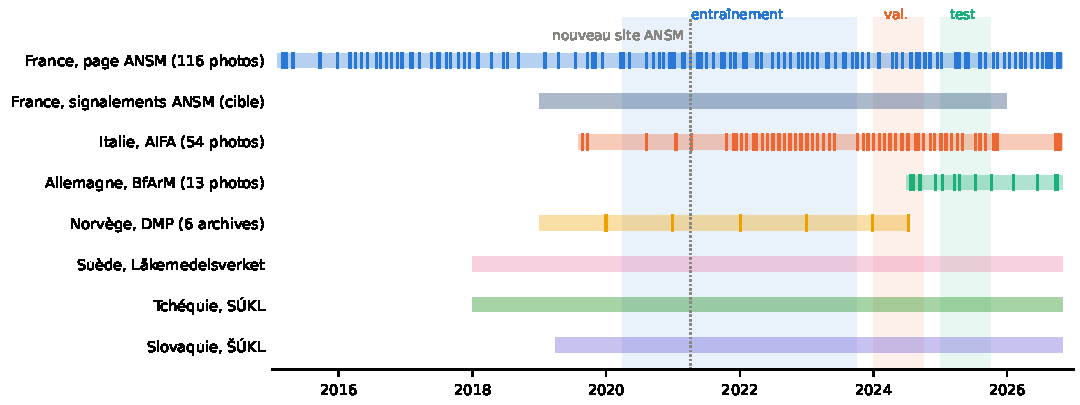
\includegraphics[width=0.78\linewidth]{figures/couverture.pdf}
\vspace{-3pt}
\caption{Période couverte par chaque source, archives (traits) et fenêtre du panel.}
\end{figure}

\section{2. Réflexion et audit : la cible était trop facile}
97\,\% des positifs de 2025 concernent une substance \emph{déjà signalée} : le cumul des signalements passés seul donne
une AUC de 0,852 (0,856 pour le modèle complet). Les signaux européens paraissent forts en brut (58\,\% de positifs si
déclaration en Suède, contre 26\,\%) mais l'historique français les explique presque entièrement. \textbf{Direction
retenue} : une cible « nouvelles pénuries », limitée aux substances calmes depuis 6 ou 12 mois (27\,718 lignes, 9,1\,\%
de positives), seul cadre où Q1 et Q2 peuvent se tester, en comparant les modèles avec et sans variables « voisins » et
« Europe ». Limite : 587 nouvelles ruptures à l'entraînement, 84 au test.

\section{3. Avancement du dashboard (livrable 2)}
Application Dash de 7 vues, sans données brutes (4\,Mo de résumés), avec des graphiques choisis selon la nature des
données : \textbf{carte de l'Europe} et frise de couverture ; \textbf{séries temporelles} (indice 2022 = 100) et carte
de saisonnalité ; \textbf{arbre ATC} lié à une \textbf{carte de chaleur} sous-classe $\times$ mois ; \textbf{boîtes et
courbes cumulées en échelle log} pour les durées ; \textbf{Gantt} par substance ; \textbf{corrélations de Spearman} ;
vue panel et qualité (absences en gris, jamais en zéro).

\section{4. Premiers tests de modèles}
Découpage temporel (test 2025). Régression logistique, arbres, forêts, boosting, Naive Bayes et SVM tournent ; les
modèles simples font aussi bien que les complexes. Cible nouvelle : AUC 0,683 sans signaux européens, 0,702 avec
(+0,019, IC 95\,\% [0,002 ; 0,037], surtout l'Italie) ; Q1 : rien de visible. \textbf{Suite :} métriques pour classes rares
(précision, rappel, F1), régression sur la durée des pénuries, rapport final.
